


\tikzset{every picture/.style={line width=0.75pt}} %set default line width to 0.75pt        

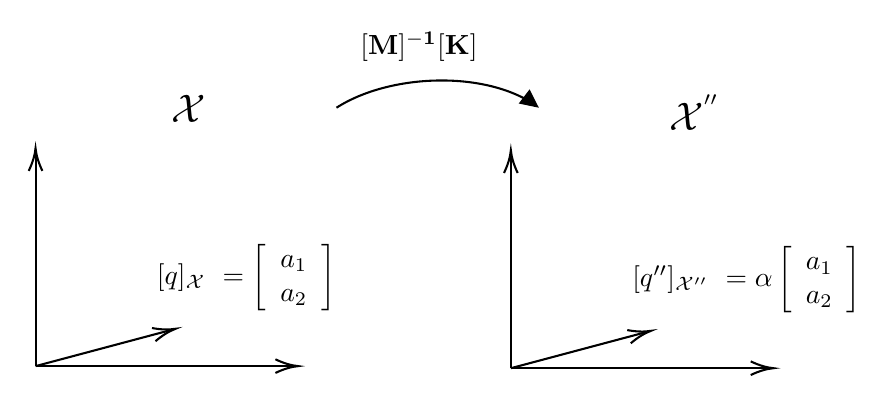
\begin{tikzpicture}[x=0.75pt,y=0.75pt,yscale=-1,xscale=1]
%uncomment if require: \path (0,15225); %set diagram left start at 0, and has height of 15225

%Straight Lines [id:da46971419391016966] 
\draw    (155,5164) -- (155,5061) ;
\draw [shift={(155,5059)}, rotate = 90] [color={rgb, 255:red, 0; green, 0; blue, 0 }  ][line width=0.75]    (10.93,-3.29) .. controls (6.95,-1.4) and (3.31,-0.3) .. (0,0) .. controls (3.31,0.3) and (6.95,1.4) .. (10.93,3.29)   ;
%Straight Lines [id:da03406383173301375] 
\draw    (155,5164) -- (279.5,5164) ;
\draw [shift={(281.5,5164)}, rotate = 180] [color={rgb, 255:red, 0; green, 0; blue, 0 }  ][line width=0.75]    (10.93,-3.29) .. controls (6.95,-1.4) and (3.31,-0.3) .. (0,0) .. controls (3.31,0.3) and (6.95,1.4) .. (10.93,3.29)   ;
%Straight Lines [id:da495111073609535] 
\draw    (155,5164) -- (220.57,5146.52) ;
\draw [shift={(222.5,5146)}, rotate = 165.07] [color={rgb, 255:red, 0; green, 0; blue, 0 }  ][line width=0.75]    (10.93,-3.29) .. controls (6.95,-1.4) and (3.31,-0.3) .. (0,0) .. controls (3.31,0.3) and (6.95,1.4) .. (10.93,3.29)   ;
%Curve Lines [id:da4396149957962707] 
\draw    (300,5039.5) .. controls (325.71,5023.01) and (371.17,5021.57) .. (395.32,5037.93) ;
\draw [shift={(397.5,5039.5)}, rotate = 217.45] [fill={rgb, 255:red, 0; green, 0; blue, 0 }  ][line width=0.08]  [draw opacity=0] (8.93,-4.29) -- (0,0) -- (8.93,4.29) -- cycle    ;
%Straight Lines [id:da12429100250589431] 
\draw    (384,5165) -- (384,5062) ;
\draw [shift={(384,5060)}, rotate = 90] [color={rgb, 255:red, 0; green, 0; blue, 0 }  ][line width=0.75]    (10.93,-3.29) .. controls (6.95,-1.4) and (3.31,-0.3) .. (0,0) .. controls (3.31,0.3) and (6.95,1.4) .. (10.93,3.29)   ;
%Straight Lines [id:da011617708076129607] 
\draw    (384,5165) -- (508.5,5165) ;
\draw [shift={(510.5,5165)}, rotate = 180] [color={rgb, 255:red, 0; green, 0; blue, 0 }  ][line width=0.75]    (10.93,-3.29) .. controls (6.95,-1.4) and (3.31,-0.3) .. (0,0) .. controls (3.31,0.3) and (6.95,1.4) .. (10.93,3.29)   ;
%Straight Lines [id:da8611613220381794] 
\draw    (384,5165) -- (449.57,5147.52) ;
\draw [shift={(451.5,5147)}, rotate = 165.07] [color={rgb, 255:red, 0; green, 0; blue, 0 }  ][line width=0.75]    (10.93,-3.29) .. controls (6.95,-1.4) and (3.31,-0.3) .. (0,0) .. controls (3.31,0.3) and (6.95,1.4) .. (10.93,3.29)   ;

% Text Node
\draw (219,5032) node [anchor=north west][inner sep=0.75pt]  [font=\Large]  {$\mathcal{X}$};
% Text Node
\draw (212,5104) node [anchor=north west][inner sep=0.75pt]    {$[ q]_{\mathcal{X}} \ =
\left[
\begin{array}{c}
a _{1}\\
a _{2}
\end{array} 
\right]  $};
% Text Node
\draw (310,5001.5) node [anchor=north west][inner sep=0.75pt]    {$\mathbf{[M]^{-1}}\mathbf{[K]}$};
% Text Node
\draw (441,5105) node [anchor=north west][inner sep=0.75pt]    {$[ q'']_{\mathcal{X} ''} \ =\alpha \left[
\begin{array}{c}
a _{1}\\
a _{2}
\end{array} 
\right]  $};
% Text Node
\draw (459,5032) node [anchor=north west][inner sep=0.75pt]  [font=\Large]  {$\mathcal{X}^{''}$};


\end{tikzpicture}
